\section{Blocks inside the MultiChain}
A peer will have transactions with other peers in the network.
The peer will want to increase his reputation and have a transaction transcribing his contribution.
The transaction contains the information about how much data was uploaded and downloaded between the peers
and their total upload and download amounts.

The transaction will be stored inside a single block.
The blocks are linked to previous blocks by adding the hashes of the previous blocks of both peers.
This creates a directed acyclic graph of blocks.
A chain can be identified within this graph for every peer.
This chain contains every transaction of a peer.

Every peer in Dispersy has a public and private key that can be used to identify them.
A block contains both public keys of the peers,
so it is possible to see to which peers the transaction belongs to.
Both peers sign the whole block using their private keys to acknowledge that the transaction has happened.
Every block only contains one transaction.

\subsection{Irrevocable proof-of-help}
Digital signatures have the property to be non-repudiable of origin \cite{VanderLubbe-crypto}.
After signing a block the signer cannot later deny providing his signature.
Only in the possesion of a secret key can a signature be made,
so only the signer could have made the signature.
This is assuming the secret key was not comprimised.

This property results in that after creating a block
both participants can no longer deny involvement in that block.
Because they cannot repudiate their own signature
The blocks become durable records aand are irrevokable and irrefutable.

\subsection{Example}

An example of three blocks can be seen in Figure \ref{fig:chain-example}.
The arrows denote that something is hashed or signed.
In this example the first block contains a transaction between peer B and C.
The block contains hashes to the previous blocks of both B and C
and can be seen by the outward arrows.
Inside the block it can be seen what part peer B and C signs by the boxes.
The whole block is not signed by both parties.
The reason for this is explained in section \ref{design:block_creation}.

In the example both peer B and C also conduct a transaction with another peer, A and D respectively.
This creates two new blocks and are chained to the block between B and C by adding the previous hash to the new blocks.
This previous hash is now the same for both B and C and the chains can be seen to be intertwined at that point.
The new blocks also contains the previous hashes of A and D
and chain the new block to previous blocks of A and D and their chains.

\begin{figure}
	\centerline{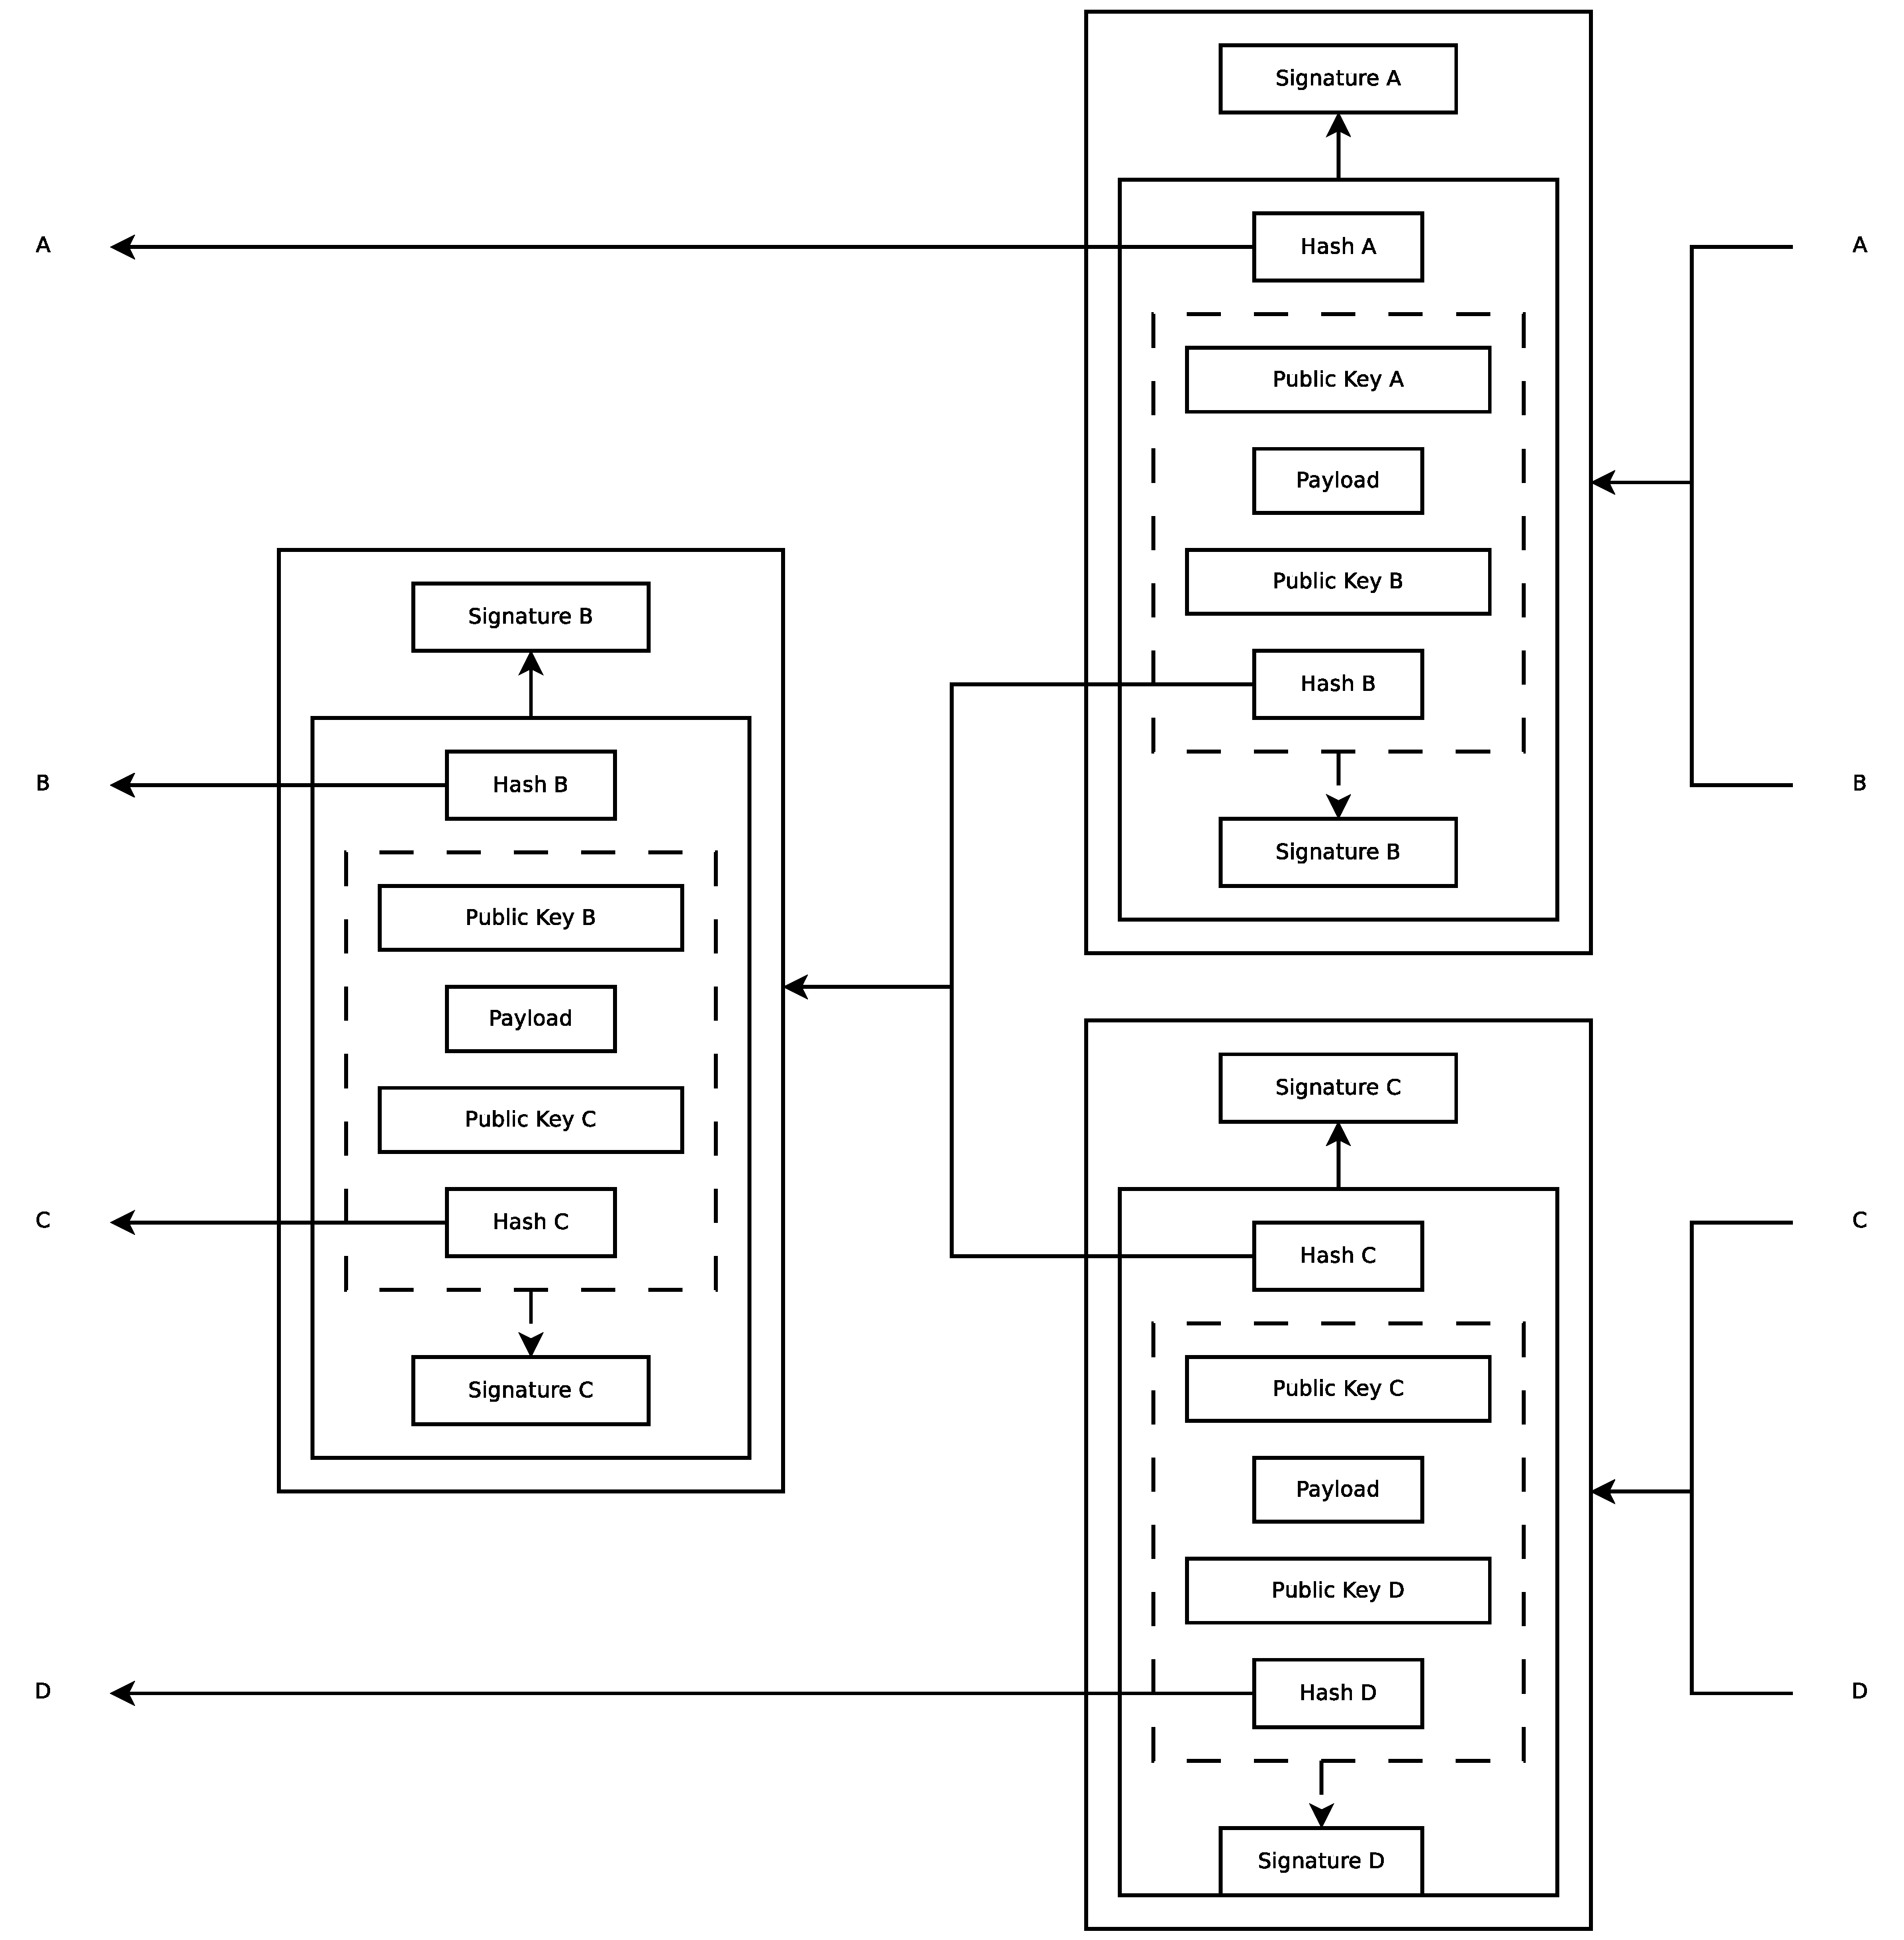
\includegraphics[scale=0.3]{design/figs/chain.eps}}
	\caption{Example of three blocks in the chain.}
	\label{fig:chain-example}
\end{figure}